\chapter{Nonlinear Time Reversal}
\label{ch:nltr}

\section{Purpose and Conceptual Overview of Nonlinear Time Reversal}
\label{sec:nltr-purpose}

The preceeding chapters have been concerned with linear time reversal, or LTR, and have focused primarily on investigating properties of reconstructions. Now, we move into our nonlinear/NLTR investigations, which focus on proof of concept of targeting capabilities. As a reminder, NLTR makes use of harmonic reflections from the target to isolate it via frequency domain inspection after the sona is collected, a process similar to how we would envision a TR based WPT system to work. 

Conceptually, our general process is this: we broadcast a Gaussian pulse from one port serving as both the transmitter and the receiver. Elsewhere in the Gigabox is a nonlinear element serving as a target. Any reflections from this element will contain harmonics: frequency components at multiples of the original frequency. These harmonics are embedded along with all the other echos in sona collected back at the transceiving port. However, before time reversing the sona, we transform it into the frequency domain and filter out all the components not within some band of the harmonic frequencies. In this way, we isolate only those wave paths that had contact with the nonlinear target. That filtered sona is time reversed and rebroadcast from the transceiving port, which will cause a slightly distorted version of the original Gaussian pulse to reconstruct at the target. This process is illustrated in Figure~\ref{fig:nonlinear-diagram}.

\begin{figure}[h!]
\centering
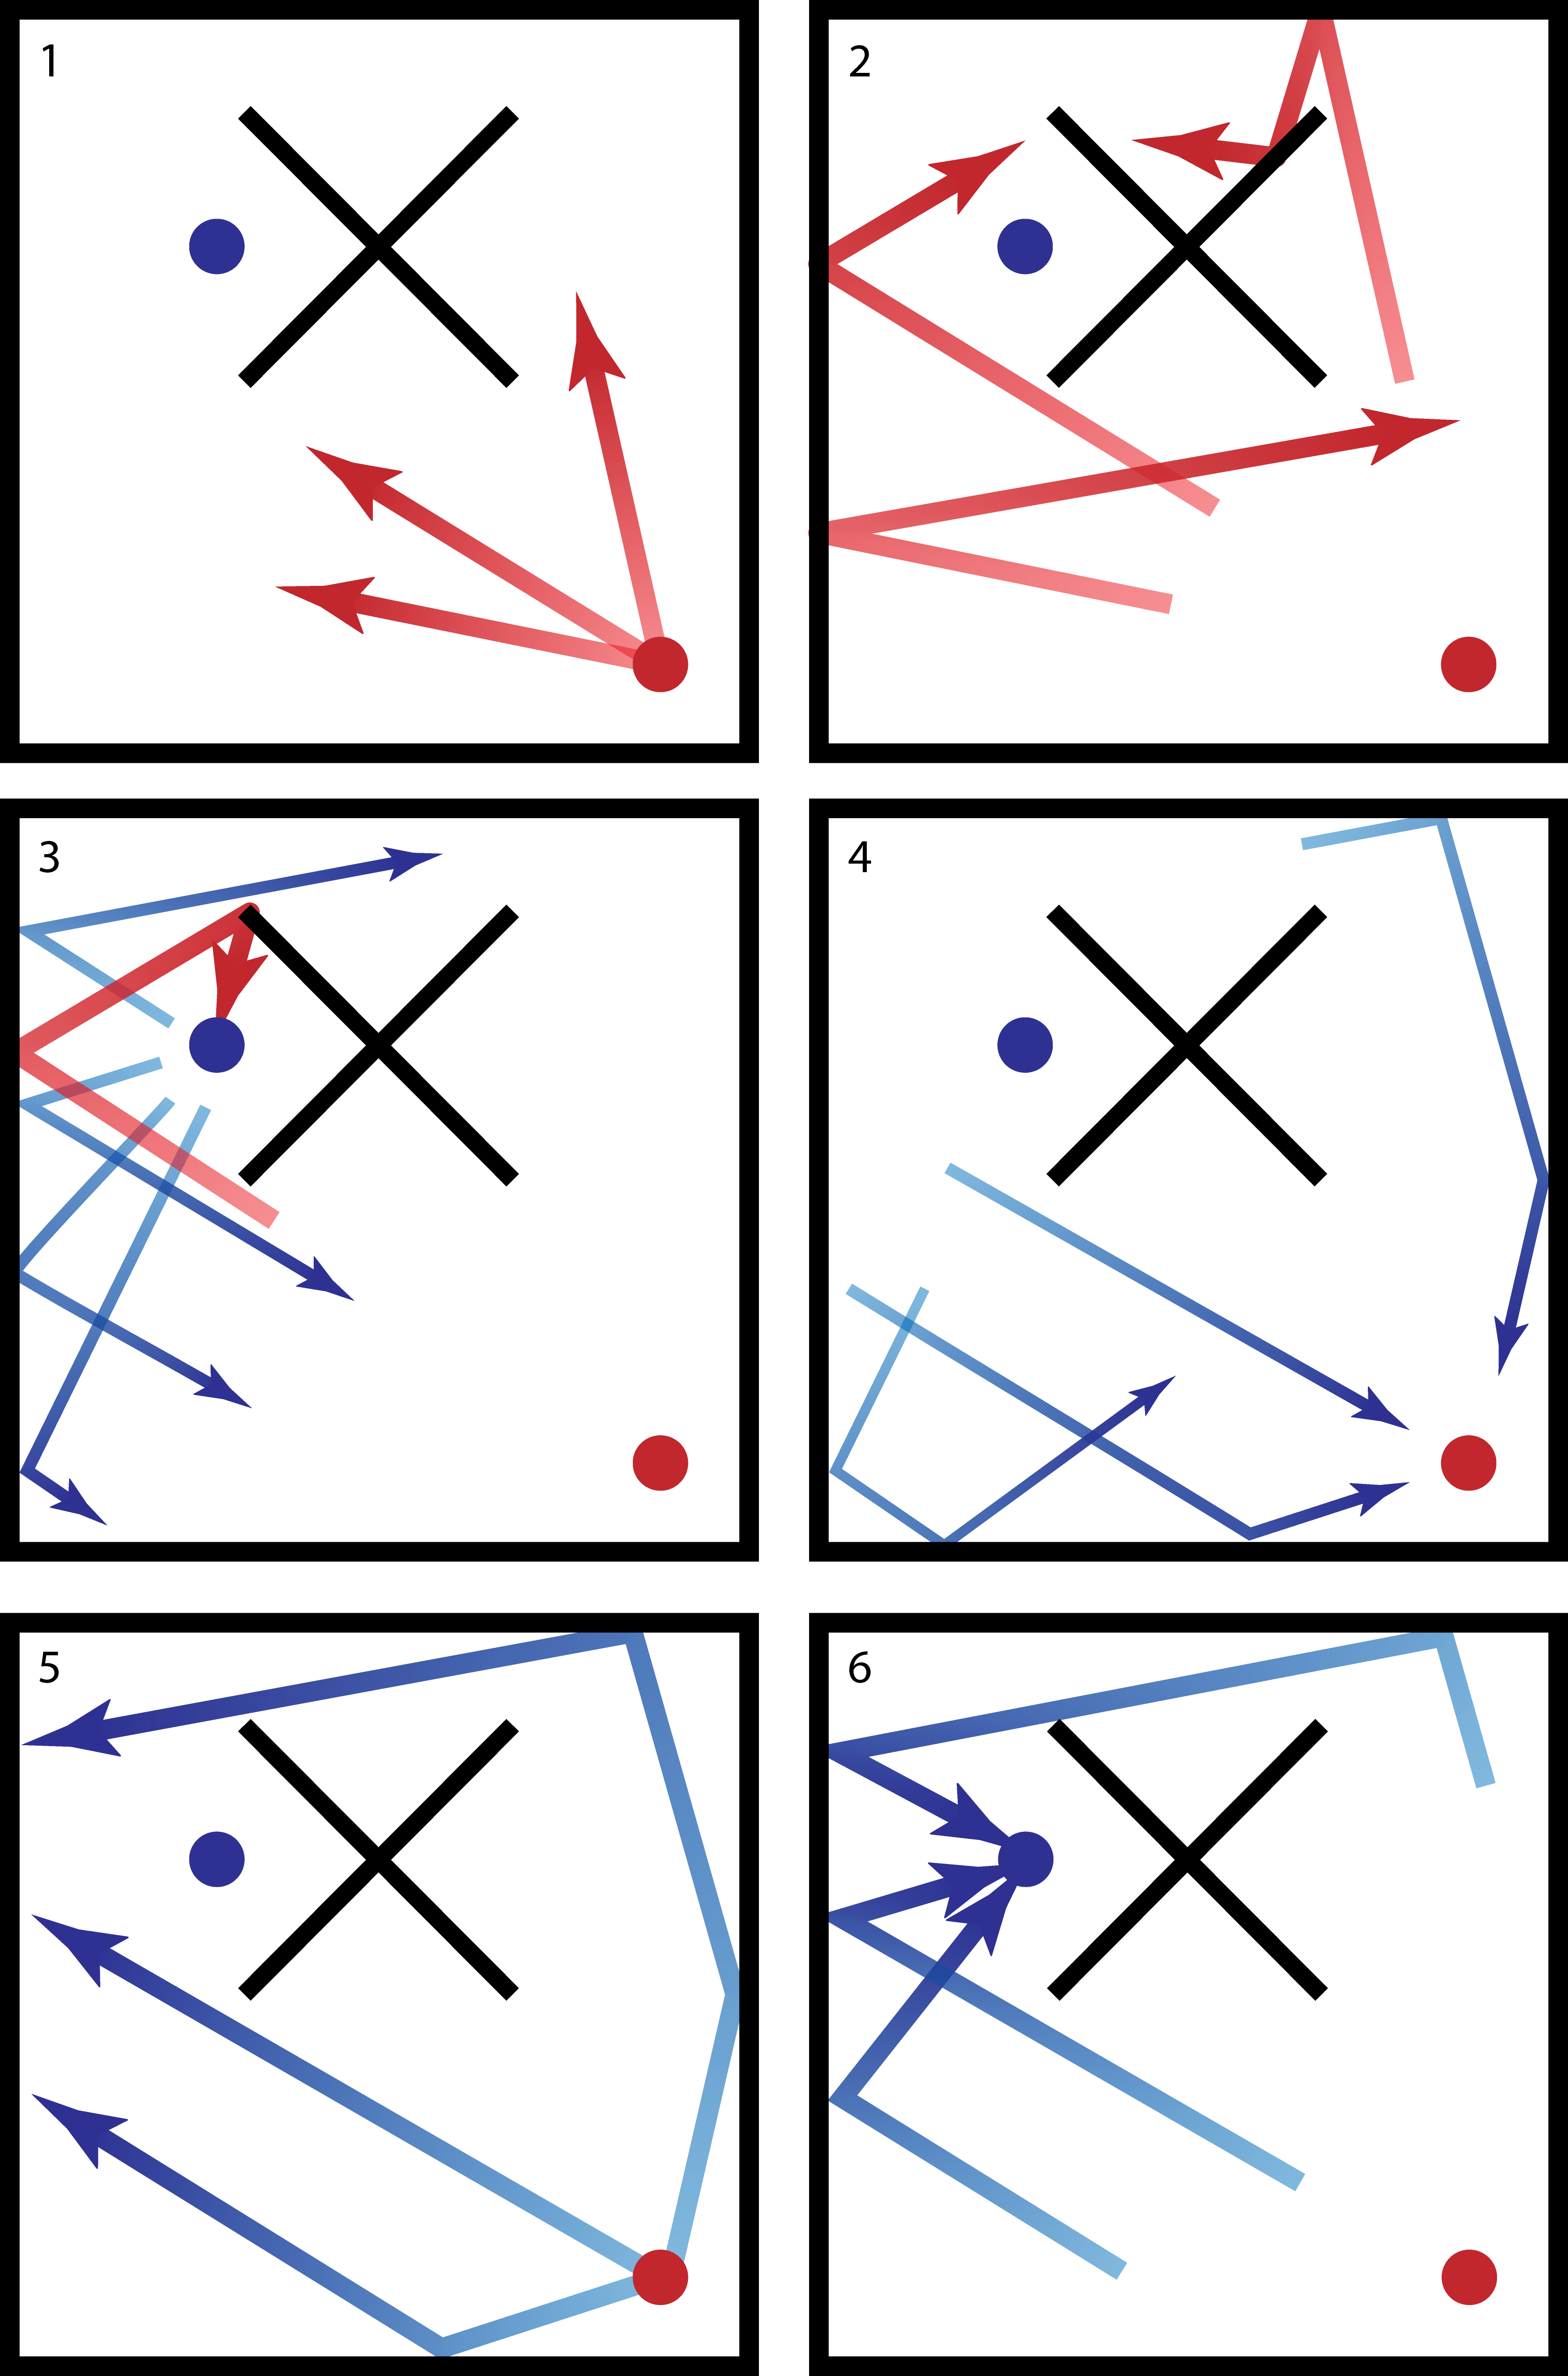
\includegraphics[width=0.85\textwidth]{nonlinear/diagram}
    \caption[Conceptual overview of nonlinear time reversal]{Reading order from top left: (1) The TRM broadcasts a signal into the cavity at one frequency, which (2) reverberates within the cavity. Eventually, (3) the signal reaches the nonlinear element somewhere within the chamber. Reflected waves that encounter this element will have a characteristic frequency signature containing harmonics of the original signal. (4) Some of these harmonic reflections will find their way back to the TRM. the TRM filters the sona to extract only those reflections, then time reverses and (5) re-emits them. (6) The time reversed waves collapse back on the nonlinear target.}
    \label{fig:nonlinear-diagram}
\end{figure}

We explored several different applications of NLTR with an eye towards adapting the technique for WPT, both experimentally and in simulation. The experimental portions met with limited success due to the diffculty of passively producing harmonics of significant magnitude. However, we believe the the applications of NLTR as a WPT method remains feasible. Discussion of the difficulties that set back our work will be presented in the "Future Works" section in the Conclusion. Successful results, including those of numerical simulations, are explored at length in the following NLTR sections. 
